\documentclass[12pt, flegn, leqno]{article}

\usepackage[utf8]{inputenc}
\usepackage[T1]{fontenc}
\usepackage{polski}

\usepackage[fleqn]{amsmath}
\usepackage{graphicx}
\usepackage[fleqn]{mathtools}

\usepackage{ulem}
\usepackage{titlesec}
\newcommand{\sectionbreak}{\clearpage} %section new page
\usepackage[labelformat=empty]{caption}
\usepackage[margin=1in, top=0.75in]{geometry}
\usepackage{setspace}
\usepackage{interval}
\usepackage{enumitem}

% augmented bmatrix
\makeatletter
\renewcommand*\env@matrix[1][*\c@MaxMatrixCols c]{%
  \hskip -\arraycolsep
  \let\@ifnextchar\new@ifnextchar
  \array{#1}}
\makeatother
 
\title{
    \Huge \textbf{Raport - temat 1} \linebreak
    \\[2pt]
    \LARGE 
    \uline{Układy równań liniowych i nieliniowych. \newline
    Zera wielomianów.} \\[5mm]
    Zadanie 5 
}
\date{17.10.2018}
\author{Przemysław Wiczołek \\ gr. F3}

\begin{document}
    \pagenumbering{gobble} % skip site number
    \maketitle
    \newpage
    \pagenumbering{arabic}
    \titlelabel{\thetitle.\quad} % dot after section number

    \section{Wstęp teoretyczny}
        \paragraph{Treść zadania:}
        \textit{Rozwiązanie układu równań w dziedzinie zespolonej. Wyjściowy układ
        sprowadzamy do układu o  elementach rzeczywistych i rozwiązujemy go metodą
        eliminacji Gaussa z częściowym wyborem elementu głównego.} \\[5mm]
        Układ równań $Ax = b$ można sprowadzić do układu rzeczywistego w podany sposób:
        \begin{gather*}
            \begin{cases}
                A = B + iC &\\
                x = y + iz &\\
                b = c + id &
            \end{cases} \\
            \implies \hspace{10mm} (B+iC)(y+iz) = c + id \\
            \implies By - Cz + iBz + iCy  = c + id 
        \end{gather*} 
        Co daje:
        \begin{gather*}
            \begin{cases}
                By - Cz = c &\\
                Bz + Cy = d &
            \end{cases}
        \end{gather*}
        A więc zwykły układ równań liniowych w dziedzinie rzeczywistej.

        \paragraph{}
        Następnie można posłużyć się metodą eliminacji Gaussa z częściowym wyborem,
        to znaczy przy każdej iteracji metody wybieramy wiersz $k$ o maksymalnej wartości
        w kolumnie $j$, a potem zamieniamy $j$-ty wiersz z $k$-tym:
        \[
            \textbf{max =>}
            \begin{bmatrix}[cccc|c]
                a_{11} & a_{12} & \cdots & a_{1n} & b_{1}\\
                \vdots & \vdots & \ddots & \vdots & \vdots\\
                a_{i1} & a_{i2} & \cdots & a_{in} & b_{i}\\
                \vdots & \vdots & \ddots & \vdots & \vdots\\
                a_{n1} & a_{n2} & \cdots & a_{nn} & b_{n}
            \end{bmatrix}
            \implies
            \begin{bmatrix}[cccc|c]
                a_{i1} & a_{i2} & \cdots & a_{in} & b_{i}\\
                \vdots & \vdots & \ddots & \vdots & \vdots\\
                a_{11} & a_{12} & \cdots & a_{1n} & b_{1}\\
                \vdots & \vdots & \ddots & \vdots & \vdots\\
                a_{n1} & a_{n2} & \cdots & a_{nn} & b_{n}
            \end{bmatrix}
        \]
        Potem wykonujemy eliminację:
        \[
            \begin{bmatrix}[cccc|c]
                a_{i1} & a_{i2}& \cdots & a_{in} & b_{i}\\
                0 & a_{22} - a_{21}/a_{i1} * a_{i2} & \cdots & a_{2n} - a_{21}/a_{i1} * a_{in} & b_{2} - a_{21}/a_{i1} * b{i}\\
                \vdots & \vdots & \ddots & \vdots\\
                0 & a_{n2} - a_{n1}/a_{i1} * a_{i2} & \cdots & a_{nn} - a_{n1}/a_{i1} * a_{in} & b_{n} - a_{n1}/a_{i1} * b{i}
            \end{bmatrix}
        \]
        \[
            \implies \cdots \implies
            \begin{bmatrix}[cccc|c]
                a_{i1} & a_{i2}& \cdots & a_{in} & b_{i}\\
                0 & * & \cdots & * & *\\
                \vdots & \vdots & \ddots & \vdots\\
                0 & 0 & \cdots & * & *
            \end{bmatrix}
        \] 
    
    \section{Opis metody}
        \subsection*{Sposób implementacji}
            \paragraph{}
            Implementacja została przeprowadzona w języku Matlab.
            Kod został rozdzielony na 
            dwie\footnote{Właściwie cztery - dwie dla GEPP w języku C i analogicznie dla Matlaba}
            funkcje: \textit{GEPP\_cmplx(A,b)} oraz \textit{GEPP(A,b)}.
            Testowanie odbywało się w skrypcie \textit{rand\_examples.m} z wykorzystaniem losowej macierzy 
            $1200 \times 1200$ z wartościami zespolonymi $z = a + bi$, 
            gdzie $a,b \in \interval{10^{-6}}{10^{6}}$. 
            \paragraph{}
            Funkcja \textit{GEPP(A,b)}, czyli funkcja obliczająca wynik równania metodą eliminacji
            Gaussa z częściowym wyborem została zaimplementowana zarówno w języku Matlab jak i 
            w C w celu porównania szybkości obliczania i dokładności wyników.
            \paragraph{}
            Funkcja \textit{GEPP\_cmplx(A,b)} została napisana w języku Matlab, ale była
            oddzielna dla obu implementacji, ze względu na niemożnośc przekazywania argumentów pionowych 
            w do funkcji w języku C. Sprowadzała ona podany układ do dziedziny rzeczywistej i wywoływała 
            funkcję GEPP do dalszych obliczeń, a później zwracała wynik.
            Była to główna funkcja programu.
            \paragraph{}
            W skrypcie \textit{time\_graph.m} został zamieszczony wykres rozmiaru macierzy do
            czasu.


        \subsection*{Warunki stopu}
            Program nie zostanie wykonany, jeżeli:
            \begin{itemize}
                \item{Ilość argumentów wejściowych lub wyjściowych jest niewłaściwa}
                \item{Macierz A nie jest kwadratowa}
                \item{Rozmiar wektora b jest inny niz rozmiar macierzy A}
                \item{Wyznacznik macierzy A jest bliski zeru}
            \end{itemize}

            
    \section{Wyniki}
        \subsection*{Dokładność}
        \begin{figure}[!h]
            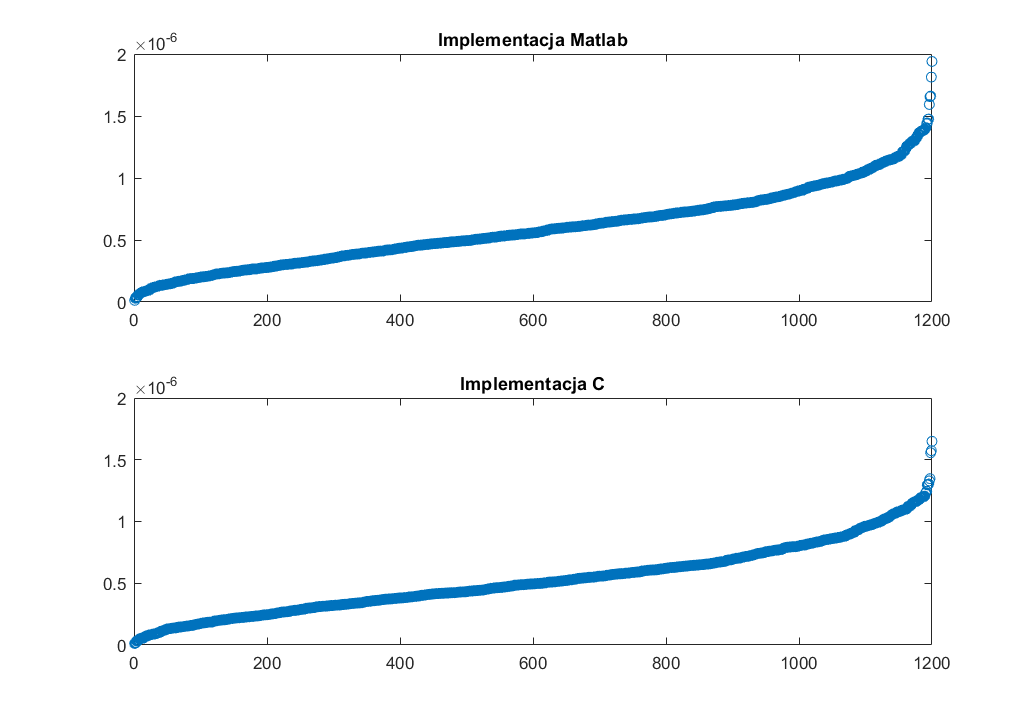
\includegraphics[width=\linewidth]{graph.png}
            \caption{Posortowane wektory błędu bezwzględnego}
            \label{fig:graph0}
        \end{figure}
        Jak można zobaczyć na wykresie błąd w wyniku jest rzędu $10^{-6}$ dla obu implementacji.
        Wynika z tego, że w domyślnej implementacji Matlab korzysta z podobnego kodowania 
        liczb zmiennoprzecinkowych jak język C.

        \newpage
        \subsection*{Czas}
        \begin{figure}[!ht]
            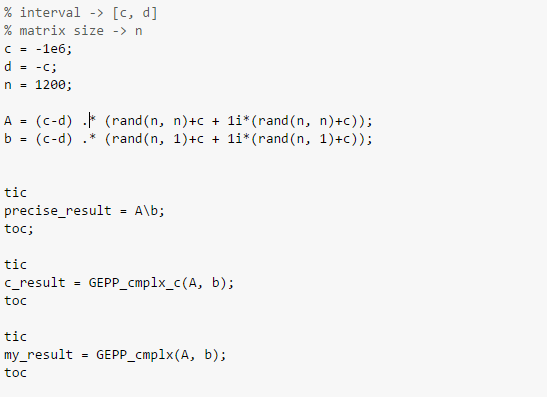
\includegraphics[width=\linewidth]{code.png}
            \caption{Kod skryptu do testów}
            \label{fig:code1}
        \end{figure}

        \begin{figure}[!ht]
            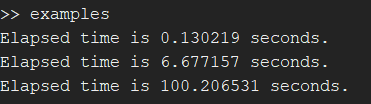
\includegraphics[width=\linewidth]{time.png}
            \caption{Czas wykonania poszczególnych funkcji}
            \label{fig:time1}
        \end{figure}

        Jak widać moja implementacja w języku C jest około \textbf{15} razy szybsza od tej samej 
        utworzonej w Matlabie. Oczywiście funkcja biblioteczna działa nieporównywalnie lepiej
        od obu moich realizacji.

        \begin{figure}[!ht]
            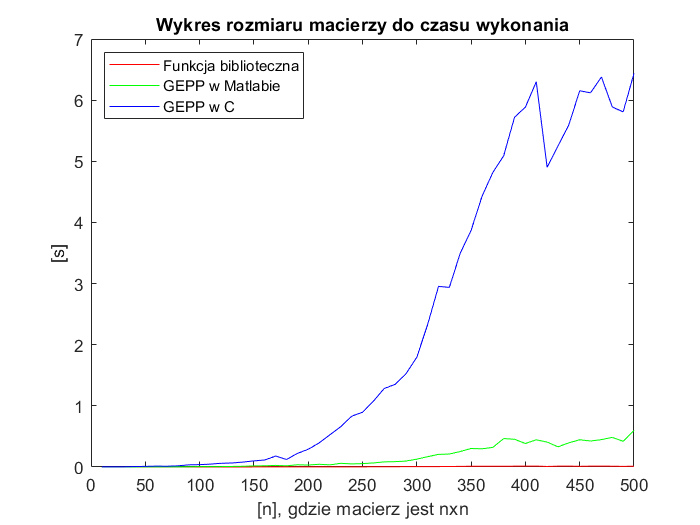
\includegraphics[width=\linewidth]{graph1.png}
            \label{fig:graph1}
        \end{figure}

        \subsection*{Przykłady obliczeniowe (również w pliku \textit{examples.m})}
            \begin{itemize}
            \item{Przykład 1}
            \begin{align*}
                A &= 
                \begin{bmatrix}
                    1.0000-0.7071i & 1.0000 - 1.4142i & 1.0000 + 0.7071i & 1.0000 - 0.2929i\\
                    1.0000+1.4142i & 2.0000 - 0.0000i & 1.0000 - 1.4142i & 2.0000 + 0.5000i\\
                    1.0000-0.7071i & 1.0000 + 1.4142i & 3.0000 + 0.7071i & 1.0000 - 1.7071i\\
                    1.0000+1.1716i & 2.0000 - 2.0000i & 1.0000 + 6.8284i & 4.0000 - 5.5000i\\
                \end{bmatrix} \\[3mm]
                b &= 
                \begin{bmatrix}
                    16.0000 + 1.0000i\\
                    5.0000 + 8.0000i\\
                    9.0000 +27.0000i\\
                    4.0000 +64.0000i\\
                \end{bmatrix} \\[3mm]
                x &= 
                \begin{bmatrix}
                    2.9100 + 1.7734i\\
                    6.1863 + 5.3519i\\
                    4.0495 + 0.0504i\\
                    -5.9409 + 0.0272i\\
                \end{bmatrix} \\[6mm] 
                &\begin{tabular}{ | l | c | c |}
                    \hline 
                    & Bład & Czas\\ \hline
                    C & 2.6922e-15 & 0.001537 s \\ \hline
                    Matlab & 3.9721e-15 & 0.005112 s \\
                    \hline
                \end{tabular}
            \end{align*}

            \item{Przykład 2}
            \begin{align*}
                A &= 
                \begin{bmatrix}
                    1.0000 + 1.0000i & 1.0000 + 0.5000i & 1.0000 + 0.3333i & 1.0000 + 0.2500i\\
                    1.0000 + 0.5000i & 2.0000 + 1.0000i & 2.0000 + 0.6667i & 2.0000 + 0.5000i\\
                    0.0000 + 0.3333i & 2.0000 + 0.6667i & 3.0000 + 1.0000i & 3.0000 + 0.7500i\\
                    0.0000 + 0.2500i & 0.0000 + 0.5000i & 3.0000 + 0.7500i & 4.0000 + 1.0000i\\
                \end{bmatrix} \\[3mm]
                b &= 
                \begin{bmatrix}
                    1.0000 - 2.0000i\\
                    0.5000 + 1.0000i\\
                    0.3333 + 0.0000i\\
                    0.2500 + 0.0000i\\
                \end{bmatrix} \\[3mm]
                x &= 
                \begin{bmatrix}
                    -1.8462 - 2.2308i\\
                    4.0933 + 2.2043i\\
                    -10.7781 - 0.8237i\\
                    8.1773 + 0.1981i\\
                \end{bmatrix} \\[6mm] 
                &\begin{tabular}{ | l | c | c |}
                    \hline 
                    & Bład & Czas\\ \hline
                    C & 1.7154e-14 & 0.000981 s \\ \hline
                    Matlab & 1.0842e-14 & 0.003475 s \\
                    \hline
                \end{tabular}
            \end{align*}

            \item{Przykład 3}
            \begin{align*}
                A &= 
                \begin{bmatrix}
                    16i  &  120i &  240i &  140i\\
                    120i & 1200i & 2700i & 1680i\\
                    240i & 2700i & 6480i & 4200i\\
                    140i & 1680i & 4200i & 2800i\\
                \end{bmatrix} \\[3mm]
                b &= 
                \begin{bmatrix}
                    1\\
                    2\\
                    3\\
                    4\\
                \end{bmatrix} \\[3mm]
                x &= 
                \begin{bmatrix}
                    4i     \\
                    2.7167i\\
                    2.1i   \\
                    1.7214i\\
                \end{bmatrix} \\[6mm] 
                &\begin{tabular}{ | l | c | c |}
                    \hline 
                    & Bład & Czas\\ \hline
                    C & 2.3981e-14 & 0.000214 s \\ \hline
                    Matlab & 2.0872e-14 & 0.000320 s \\
                    \hline
                \end{tabular}
            \end{align*}
            \end{itemize}

    \section{Podsumowanie}
        \paragraph{}
        Po przeprowadzeniu analizy wnioskuję, że obliczenia na liczbach zespolonych w programie 
        Matlab nie są dużo bardziej skomplikowane w porównaniu do liczb rzeczywistych.\\
        \indent Oczywiście ilość danych jest zwiększona czterokrotnie w porównaniu do zwykłego układu
        równań, aczkolwiek nie wpływa to w żaden sposób na realizację samej funkcji \textit{GEPP}.
        Korzystając z funkcji bibliotecznych prawie wcale nie odczujemy różnicy w szybkości.
        \paragraph{}
        Ciekawą sprawą jest, że nawet zwektoryzowany(na miarę moich możliwości) kod w języku
        Matlab jest znacznie wolniejszy od tej samej, najprostszej implementacji w języku C.
        Prawdopodobnie wynika, to z mojej małej znajomości narzędzia MathWorks, chociaż
        nie szczycę się również dużą wiedzą o C. \\
        \indent Mam przeświadczenie, że język C jest dużo lepszym narzędziem do pisania prostych wydajnych
        implementacji, szczególnie, że MathWorks oferuje taką możliwość udostępniając swoje API.
        Nie sprawiło mi wiele trudności, żeby skorzystać z dostępnej dokumentacji, a program w C 
        właściwie nie różnił się od zwykłego.
\end{document}
